% Fano Plane PG(2,2) — The Architecture of Self-Observation
% 7 points = 7 dimensions, 7 lines = 7 observation triples

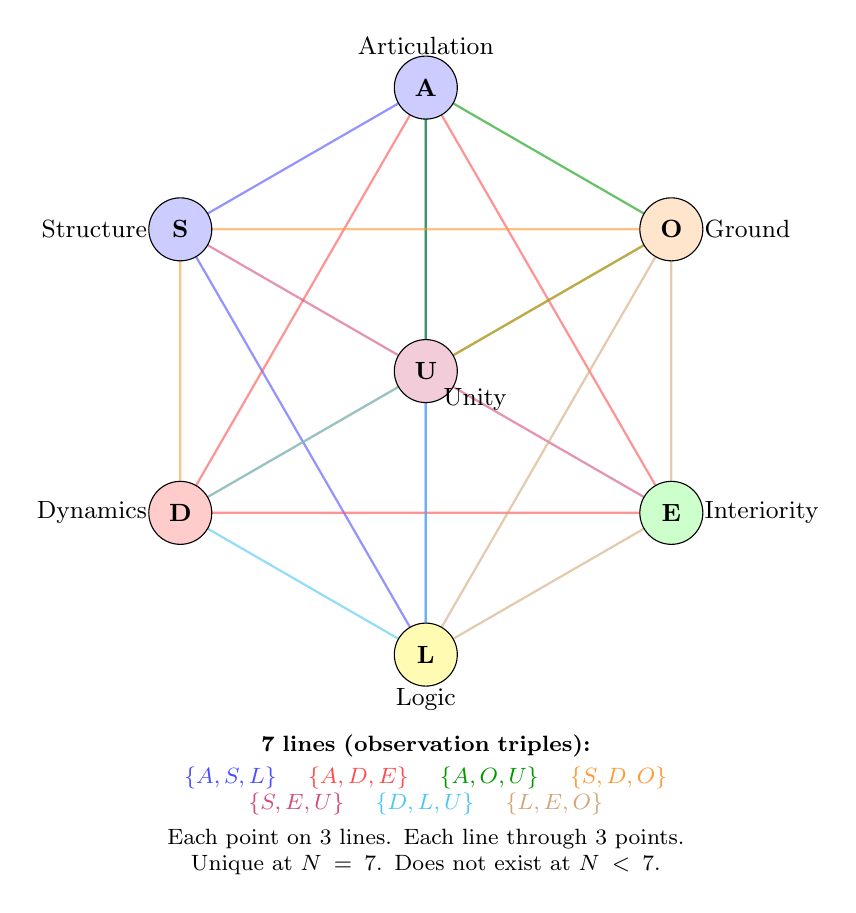
\begin{tikzpicture}[
  point/.style={circle, fill=#1, draw=black, minimum size=8mm, inner sep=0pt, font=\small\bfseries},
  line/.style={thick, #1},
  scale=1.8
]

% === Coordinates (regular hexagon + center) ===
\coordinate (A) at (90:2);     % top
\coordinate (S) at (150:2);    % upper-left
\coordinate (D) at (210:2);    % lower-left
\coordinate (L) at (270:2);    % bottom
\coordinate (E) at (330:2);    % lower-right
\coordinate (O) at (30:2);     % upper-right
\coordinate (U) at (0:0);      % center

% === Lines (7 Fano lines, drawn first so points overlay) ===
% Line 1: {A, S, L}
\draw[line=blue!70, opacity=0.6] (A) -- (S) -- (L) -- cycle;
% Line 2: {A, D, E}
\draw[line=red!70, opacity=0.6] (A) -- (D) -- (E) -- cycle;
% Line 3: {A, O, U}
\draw[line=green!60!black, opacity=0.6] (A) -- (O) -- (U) -- cycle;
% Line 4: {S, D, O}
\draw[line=orange!80, opacity=0.6] (S) -- (D) -- (O) -- cycle;
% Line 5: {S, E, U}
\draw[line=purple!70, opacity=0.6] (S) -- (E) -- (U) -- cycle;
% Line 6: {D, L, U}
\draw[line=cyan!70, opacity=0.6] (D) -- (L) -- (U) -- cycle;
% Line 7: {L, E, O} — the inscribed circle line
\draw[line=brown!70, opacity=0.6] (L) -- (E) -- (O) -- cycle;

% === Points ===
\node[point=blue!20]   at (A) {A};
\node[point=blue!20]   at (S) {S};
\node[point=red!20]    at (D) {D};
\node[point=yellow!30] at (L) {L};
\node[point=green!20]  at (E) {E};
\node[point=orange!20] at (O) {O};
\node[point=purple!20] at (U) {U};

% === Labels ===
\node[above=3mm] at (A) {\small Articulation};
\node[left=3mm]  at (S) {\small Structure};
\node[left=3mm]  at (D) {\small Dynamics};
\node[below=3mm] at (L) {\small Logic};
\node[right=3mm] at (E) {\small Interiority};
\node[right=3mm] at (O) {\small Ground};
\node[below right=1mm] at (U) {\small Unity};

% === Legend (centered) ===
\node[anchor=north, font=\footnotesize, text width=7cm, align=center] at (0, -2.5) {
  \textbf{7 lines (observation triples):}\\[2pt]
  \textcolor{blue!70}{$\{A,S,L\}$} \quad
  \textcolor{red!70}{$\{A,D,E\}$} \quad
  \textcolor{green!60!black}{$\{A,O,U\}$} \quad
  \textcolor{orange!80}{$\{S,D,O\}$}\\
  \textcolor{purple!70}{$\{S,E,U\}$} \quad
  \textcolor{cyan!70}{$\{D,L,U\}$} \quad
  \textcolor{brown!70}{$\{L,E,O\}$}\\[3pt]
  Each point on 3 lines. Each line through 3 points.\\
  Unique at $N=7$. Does not exist at $N<7$.
};

\end{tikzpicture}
